\section{Durchführung}
\label{sec:Durchführung}

\subsection{Wheatstone Brücke}
\begin{figure}[H]
    \centering
        \centering
        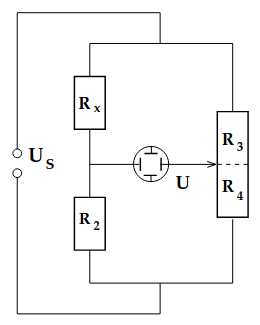
\includegraphics[width=0.35\textwidth]{Bilder/wheatstone.png}
        \caption{Wheatstone Brücke. \cite{anleitung}}
    \hfill
    \label{fig:f2}
\end{figure}
\noindent Bei der Wheatstone Brücke befinden sich nur Ohmsche Widerstände in 
dem Schaltkreis. Dabei sind $R3$ und $R4$ am Potentiometer (Spannungsteiler, 
an dem ein Schleifkontakt über den Widerstandtsdraht gelegt wird, was es
ermöglicht, den Widerstand kontinuierlich einzustellen). Um nun den unbekannten 
Widerstand $R_x$ durch die Kompensationsmethode zu bestimmen, gilt
\begin{equation}
    R_x = R_2 \frac{R_3}{R_4}.
\end{equation}
\noindent Als Einstellungen werden folgende Werte genommen:
\begin{align*}
    \label{eqn:werte1}
    \text{Spannungsteiler } R_3 \text{ und } R_4 &= 1\,k\Omega \\
    \text{Frequenz } \nu &= 1\,kHz \\
    \text{Amplitude } U_S &= 1\,V \\
    \text{Widerstand } R_2 &= 332;\, 664;\, 1000\,\Omega \\
\end{align*}


\subsection{Kapazitätsmessbrücke}
\begin{figure}[H]
    \centering
        \centering
        \includegraphics[width=0.35\textwidth]{Bilder/kapazitätsmess.png}
        \caption{Kapazitätsmessbrücke. \cite{anleitung}}
    \hfill
    \label{fig:f3}
\end{figure}
\noindent Da in diesem Bereich des Experiments Kapazitäten bestimmt werden sollen, 
muss der Wechselstrom verwendet weren.

\subsection{Induktivitätsmessbrücke}
\begin{figure}[H]
    \centering
        \centering
        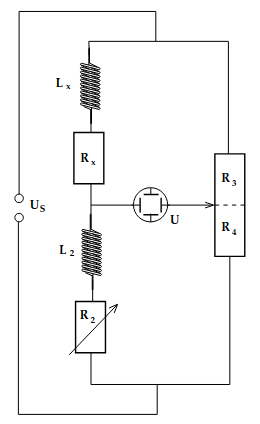
\includegraphics[width=0.35\textwidth]{Bilder/induktivitaetsmess.png}
        \caption{Induktivitätsmessbrücke. \cite{anleitung}}
    \hfill
    \label{fig:f4}
\end{figure}

\subsection{Wien-Robinson Messbrücke}
\begin{figure}[H]
    \centering
        \centering
        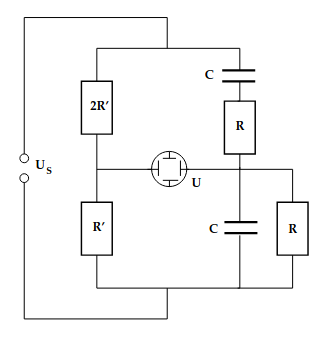
\includegraphics[width=0.35\textwidth]{Bilder/wien_robinson.png}
        \caption{Wien-Robinson Messbrücke. \cite{anleitung}}
    \hfill
    \label{fig:f5}
\end{figure}
